\documentclass[a3paper,14pt]{extarticle}
\usepackage{extsizes}
\usepackage{cmap}
\usepackage[utf8]{inputenc}
\usepackage[T2A]{fontenc}
\usepackage[english,russian]{babel} 
\usepackage[left=15mm, top=25mm, right=15mm, bottom=30mm, nohead, nofoot]{geometry}
\usepackage{graphicx}  % изобржаения
\usepackage{wrapfig}  % изобржаения
\usepackage{tikz} % графика
\usepackage{xcolor} % определение цветов
\usepackage{nicefrac} % красивые дроби
\usepackage{cancel} % сокращение
\usepackage{amsmath,amsfonts,amssymb} % математический пакет
\usepackage{hyperref}  % гиперссылки
\usepackage{fancybox,fancyhdr} % хедер и футер
\pagestyle{fancy}
\fancyhf{}
\fancyhead[L]{Практическая линейная алгебра}
\fancyhead[R]{Овчинников Павел}
\fancyfoot[C]{\thepage}
\setcounter{page}{1}
\headsep=10mm
\footskip=15mm

\definecolor{urlcolor}{HTML}{3454D1}
\definecolor{linkcolor}{HTML}{3454D1}
\hypersetup{pdfstartview=FitH, linkcolor=linkcolor, urlcolor=urlcolor, colorlinks=true}

\newlength{\tempheight}
\newcommand{\Let}{
\mathbin{\text{\settoheight{\tempheight}{\mathstrut}\raisebox{0.4\pgflinewidth}{
\tikz[baseline=0.5ex,line cap=round,line join=round] \draw (0,0) --++ (0.3em,0) --++ (0,2.3ex) --++ (-0.3em,0);
}}}}
\newcommand*\circled[1]{\tikz[baseline=(char.base)]{
            \node[shape=circle,draw,inner sep=2pt] (char) {#1};}}
\newcommand*\squared[1]{\tikz[baseline=(char.base)]{
            \node[shape=rectangle,draw,inner sep=4pt] (char) {$#1$};}}
\newcommand{\at}{\biggr\rvert}
\newcommand{\shiftright}[3]{\makebox[#2][r]{\makebox[#1][l]{#3}}}

\newcommand\NB{\textbf{N\kern-0.32em\textcolor{red}{B}}}
\newcommand{\observ}[1]{\textbf{\textit{Рубрика «наблюдения»}:} \textit{#1}}

\begin{document}
\section*{\centering Лабораторная работа №5}
\subsection*{\centering Задание №1. Е\dots\ Дружитес}
Первым делом самолёты\dots\  и, конечно, воображение, поэтому сейчас придумаем красивенький связный граф из 20 вершин. Вы легко сможете <<визуально>> выделить в нём несколько кластеров, в которых особо тесные связи. Вершины в графе уже пронумерованы. Итак, вот он, шедевр:
\begin{figure}[h]
    \centering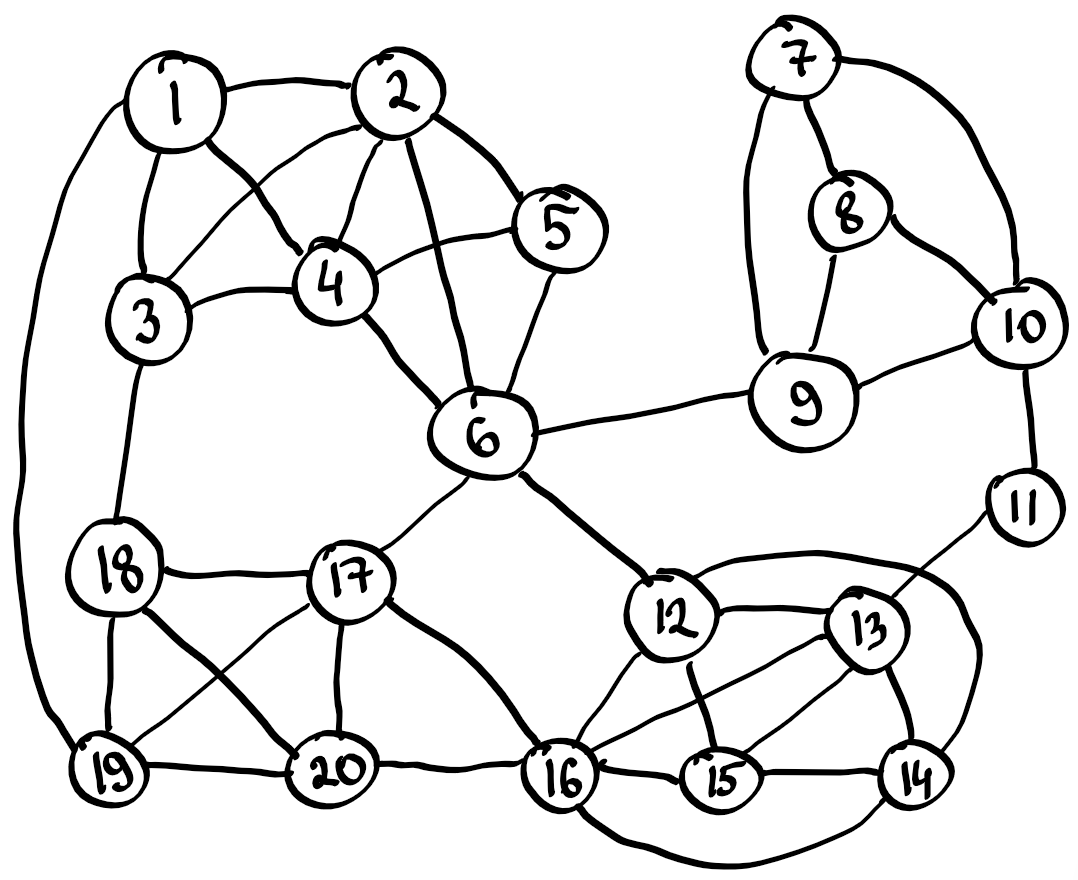
\includegraphics[width=0.4\textwidth]{1.png}
\end{figure} \\
Здесь легко выделяются 4 сообщества: вокруг \circled{4}, вокруг \circled{8}, слева снизу и вокруг \circled{15}. Остаётся вершина, наименее связанная со всеми остальными, под номером \circled{11} --- пускай этот волк-одиночка тоже выделяется в своё 5-е сообщество.\\[1em]
Теперь составим лапласиан для этого графа в соответствии с нумерацией вершин:
$$\mathcal{L} = \left[\begin{array}{rrrrrrrrrrrrrrrrrrrr}
    4 & -1 & -1 & -1 & 0 & 0 & 0 & 0 & 0 & 0 & 0 & 0 & 0 & 0 & 0 & 0 & 0 & 0 & -1 & 0 \\
    -1 & 5 & -1 & -1 & -1 & -1 & 0 & 0 & 0 & 0 & 0 & 0 & 0 & 0 & 0 & 0 & 0 & 0 & 0 & 0 \\
    -1 & -1 & 4 & -1 & 0 & 0 & 0 & 0 & 0 & 0 & 0 & 0 & 0 & 0 & 0 & 0 & 0 & -1 & 0 & 0 \\
    -1 & -1 & -1 & 5 & -1 & -1 & 0 & 0 & 0 & 0 & 0 & 0 & 0 & 0 & 0 & 0 & 0 & 0 & 0 & 0 \\
    0 & -1 & 0 & -1 & 3 & -1 & 0 & 0 & 0 & 0 & 0 & 0 & 0 & 0 & 0 & 0 & 0 & 0 & 0 & 0 \\
    0 & -1 & 0 & -1 & -1 & 6 & 0 & 0 & -1 & 0 & 0 & -1 & 0 & 0 & 0 & 0 & -1 & 0 & 0 & 0 \\
    0 & 0 & 0 & 0 & 0 & 0 & 3 & -1 & -1 & -1 & 0 & 0 & 0 & 0 & 0 & 0 & 0 & 0 & 0 & 0 \\
    0 & 0 & 0 & 0 & 0 & 0 & -1 & 3 & -1 & -1 & 0 & 0 & 0 & 0 & 0 & 0 & 0 & 0 & 0 & 0 \\
    0 & 0 & 0 & 0 & 0 & -1 & -1 & -1 & 4 & -1 & 0 & 0 & 0 & 0 & 0 & 0 & 0 & 0 & 0 & 0 \\
    0 & 0 & 0 & 0 & 0 & 0 & -1 & -1 & -1 & 4 & -1 & 0 & 0 & 0 & 0 & 0 & 0 & 0 & 0 & 0 \\
    0 & 0 & 0 & 0 & 0 & 0 & 0 & 0 & 0 & -1 & 2 & 0 & -1 & 0 & 0 & 0 & 0 & 0 & 0 & 0 \\
    0 & 0 & 0 & 0 & 0 & -1 & 0 & 0 & 0 & 0 & 0 & 5 & -1 & -1 & -1 & -1 & 0 & 0 & 0 & 0 \\
    0 & 0 & 0 & 0 & 0 & 0 & 0 & 0 & 0 & 0 & -1 & -1 & 5 & -1 & -1 & -1 & 0 & 0 & 0 & 0 \\
    0 & 0 & 0 & 0 & 0 & 0 & 0 & 0 & 0 & 0 & 0 & -1 & -1 & 4 & -1 & -1 & 0 & 0 & 0 & 0 \\
    0 & 0 & 0 & 0 & 0 & 0 & 0 & 0 & 0 & 0 & 0 & -1 & -1 & -1 & 4 & -1 & 0 & 0 & 0 & 0 \\
    0 & 0 & 0 & 0 & 0 & 0 & 0 & 0 & 0 & 0 & 0 & -1 & -1 & -1 & -1 & 6 & -1 & 0 & 0 & -1 \\
    0 & 0 & 0 & 0 & 0 & -1 & 0 & 0 & 0 & 0 & 0 & 0 & 0 & 0 & 0 & -1 & 5 & -1 & -1 & -1 \\
    0 & 0 & -1 & 0 & 0 & 0 & 0 & 0 & 0 & 0 & 0 & 0 & 0 & 0 & 0 & 0 & -1 & 4 & -1 & -1 \\
    -1 & 0 & 0 & 0 & 0 & 0 & 0 & 0 & 0 & 0 & 0 & 0 & 0 & 0 & 0 & 0 & -1 & -1 & 4 & -1 \\
    0 & 0 & 0 & 0 & 0 & 0 & 0 & 0 & 0 & 0 & 0 & 0 & 0 & 0 & 0 & -1 & -1 & -1 & -1 & 4
\end{array}\right]$$ 

\pagebreak\noindent Громадная штуковина, но отставим юмор --- нам ещё ''считать'' собственные числа и собственные вектора этой матрицы Лапласа. Для начала составим $V_{max}$, в который я положу 5 собственных векторов с минимальными собственными числами:
$$V = \left[\begin{array}{rrrrr}
    -0.224 & -0.193 & -0.234 & -0.069 & -0.086 \\
    -0.224 & -0.161 & -0.241 & -0.254 & -0.009 \\
    -0.224 & -0.193 & -0.234 & -0.069 & -0.086 \\
    -0.224 & -0.161 & -0.241 & -0.254 & -0.009 \\
    -0.224 & -0.143 & -0.245 & -0.393 & 0.06 \\
    -0.224 & -0.059 & -0.103 & -0.149 & 0.091 \\
    -0.224 & 0.439 & -0.148 & 0.099 & 0.201 \\
    -0.224 & 0.439 & -0.148 & 0.099 & 0.201 \\
    -0.224 & 0.332 & -0.137 & 0.031 & 0.167 \\
    -0.224 & 0.396 & -0.067 & 0.035 & -0.125 \\
    -0.224 & 0.239 & 0.205 & -0.134 & -0.844 \\
    -0.224 & -0.052 & 0.295 & -0.129 & 0.171 \\
    -0.224 & 0.001 & 0.352 & -0.126 & -0.051 \\
    -0.224 & -0.05 & 0.385 & -0.124 & 0.195 \\
    -0.224 & -0.05 & 0.385 & -0.124 & 0.195 \\
    -0.224 & -0.083 & 0.273 & 0.048 & 0.117 \\
    -0.224 & -0.149 & 0.013 & 0.302 & 0.005 \\
    -0.224 & -0.192 & -0.076 & 0.393 & -0.085 \\
    -0.224 & -0.192 & -0.076 & 0.393 & -0.085 \\
    -0.224 & -0.168 & 0.04 & 0.425 & -0.022
\end{array}\right]$$
И ещё одна чуть менее громадная штуковина. Эта матрица полностью пригодится для кластеризации на 5 кластеров, а далее будем просто отсекать по одному вектору справа, чтобы кластеризовать на 4, 3 и 2 кластера.\\[1em]
Коротко о том, как я составил матрицу:
\begin{figure}[h]
    \centering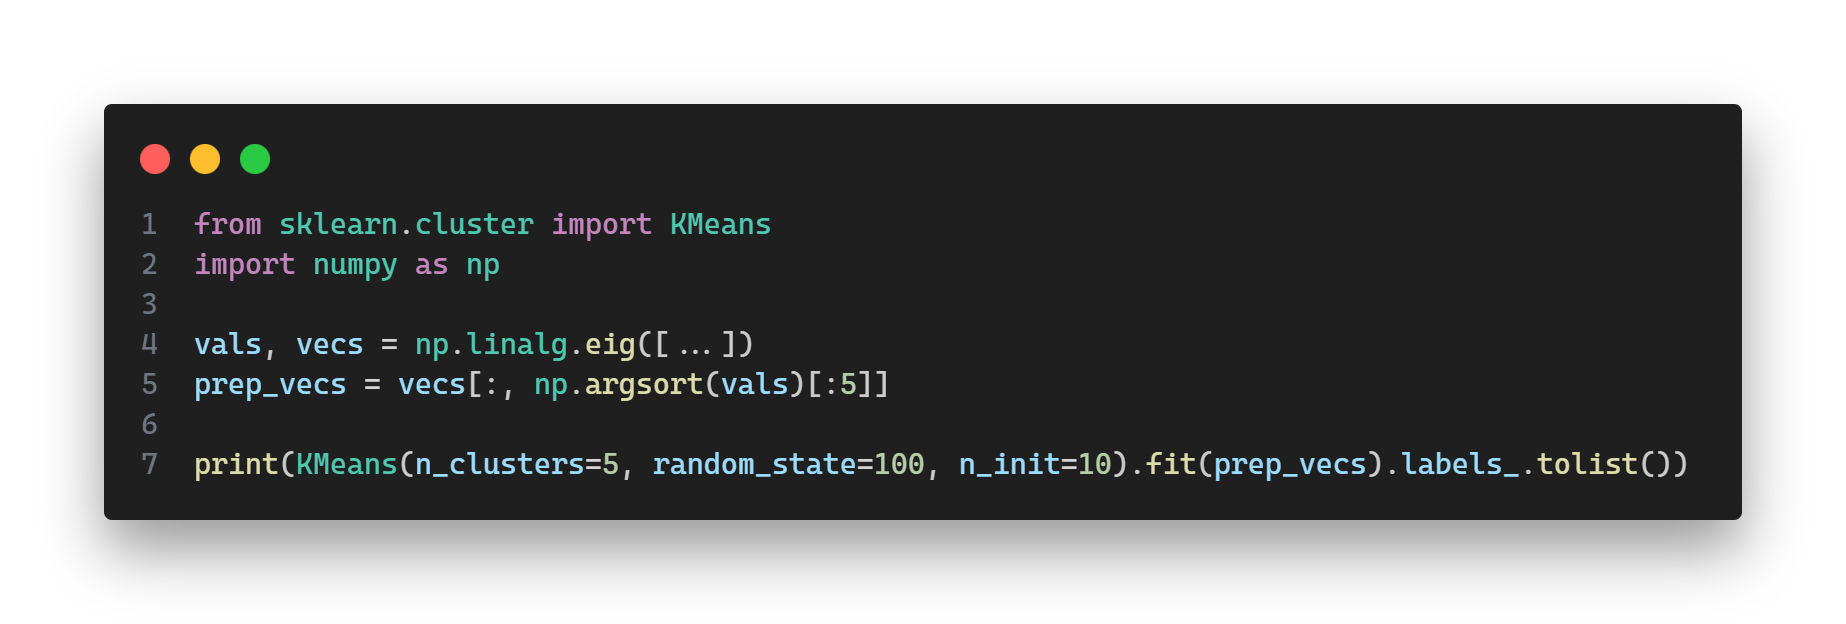
\includegraphics[width=0.7\textwidth]{1code.png}
\end{figure} \\
Просто импортируем нужные модули, подгружаем всю матрицу Лапласа в \verb|np.linalg.eig()| (заменено на эллипсис в целях экономии пространства), берём первые 5 собственных векторов по возрастанию собственных чисел, подгружаем их в \verb|KMeans| от \textbf{scikit-learn} и затем выгружаем оттуда лейблы для каждого из векторов, которые покажут, к какому кластеру принадлежит каждый из векторов.\\[1em]
Вот так выглядит разбиение на 5 кластеров ($k = 5$):
\begin{figure}[h]
    \centering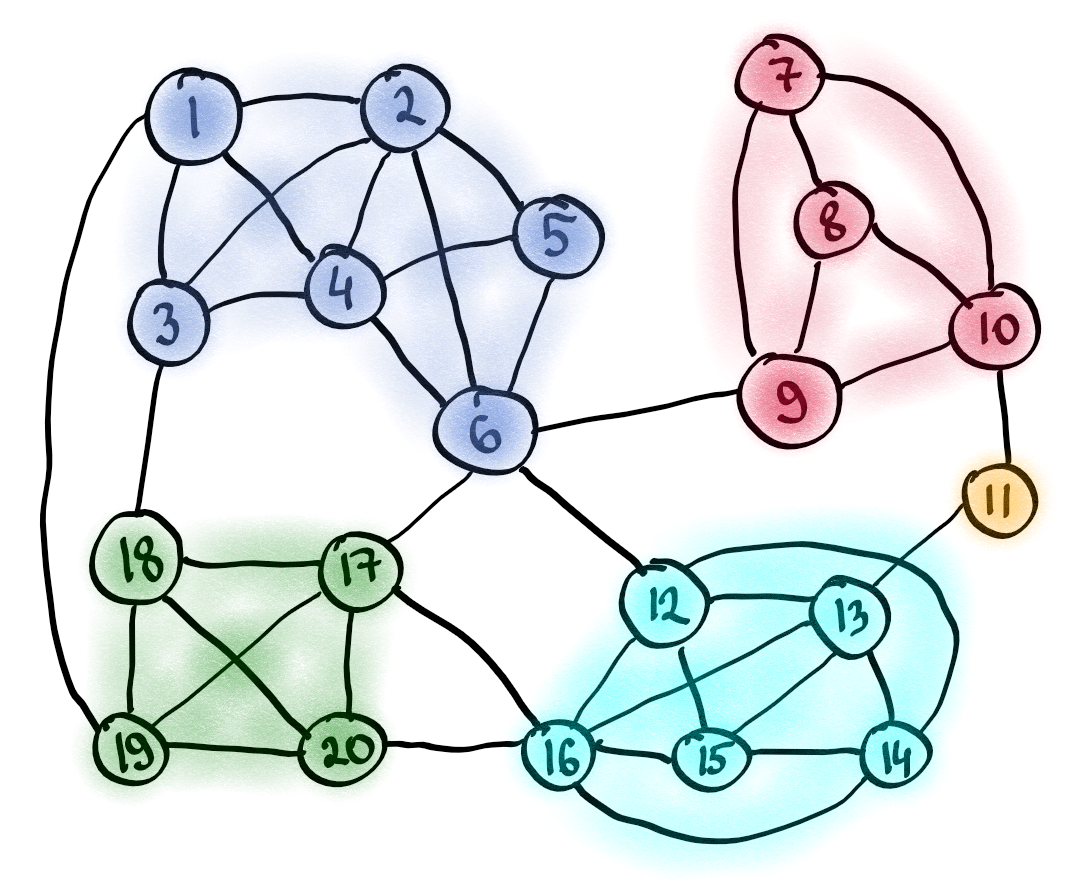
\includegraphics[width=0.4\textwidth]{1(5).png}
\end{figure} \\
Разбиение на 4 кластера несильно отличается от кластеризации на 5 блоков --- волк-одиночка \circled{11} присоединяется к более тяжёлому кластеру (кластеру с более тесными связями).
\begin{figure}[h]
    \centering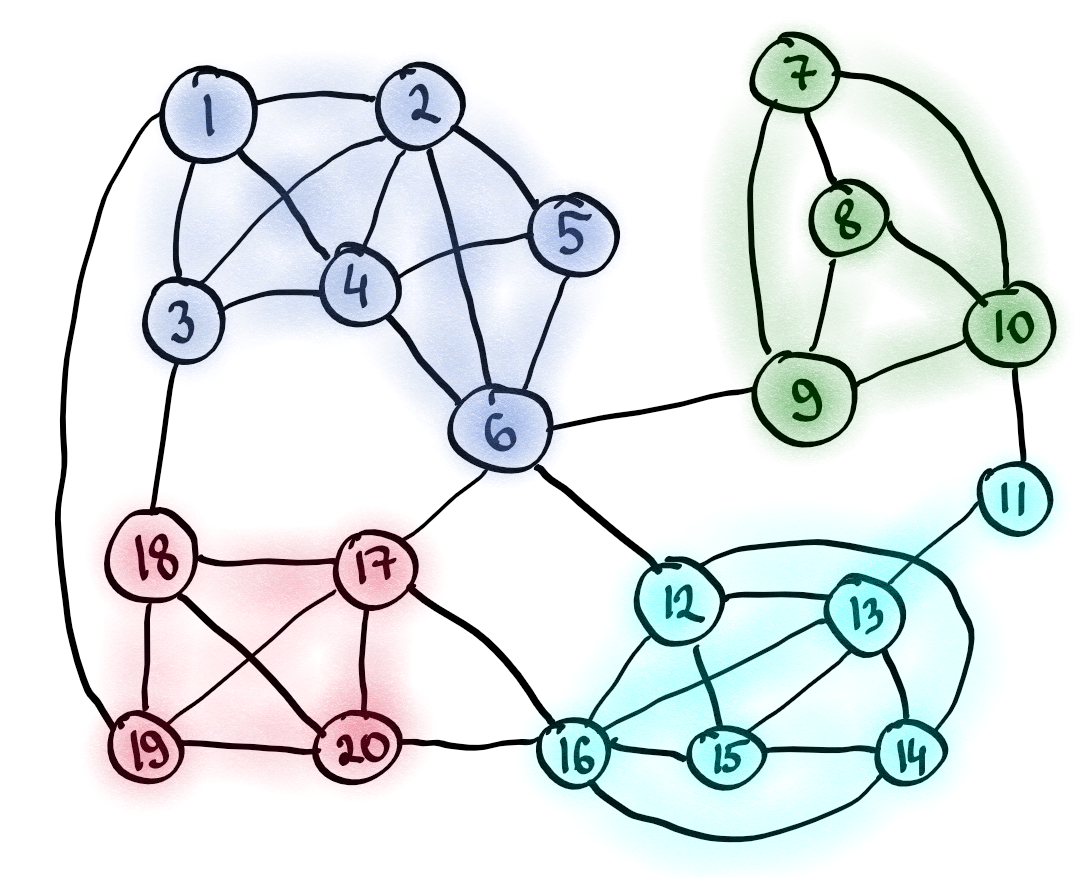
\includegraphics[width=0.4\textwidth]{1(4).png}
\end{figure} \\
Кластеризация с $k = 3$ выжимает самую слабую группу, но не (7-8-9-10), а ту, что связана наибольшим количеством вершин с более тяжёлой группой. Так кластер (17-18-19-20) был связан с (1-2-3-4-5-6) через вершины \circled{1}, \circled{3} и \circled{6}, поэтому оказался под ударом:
\begin{figure}[h]
    \centering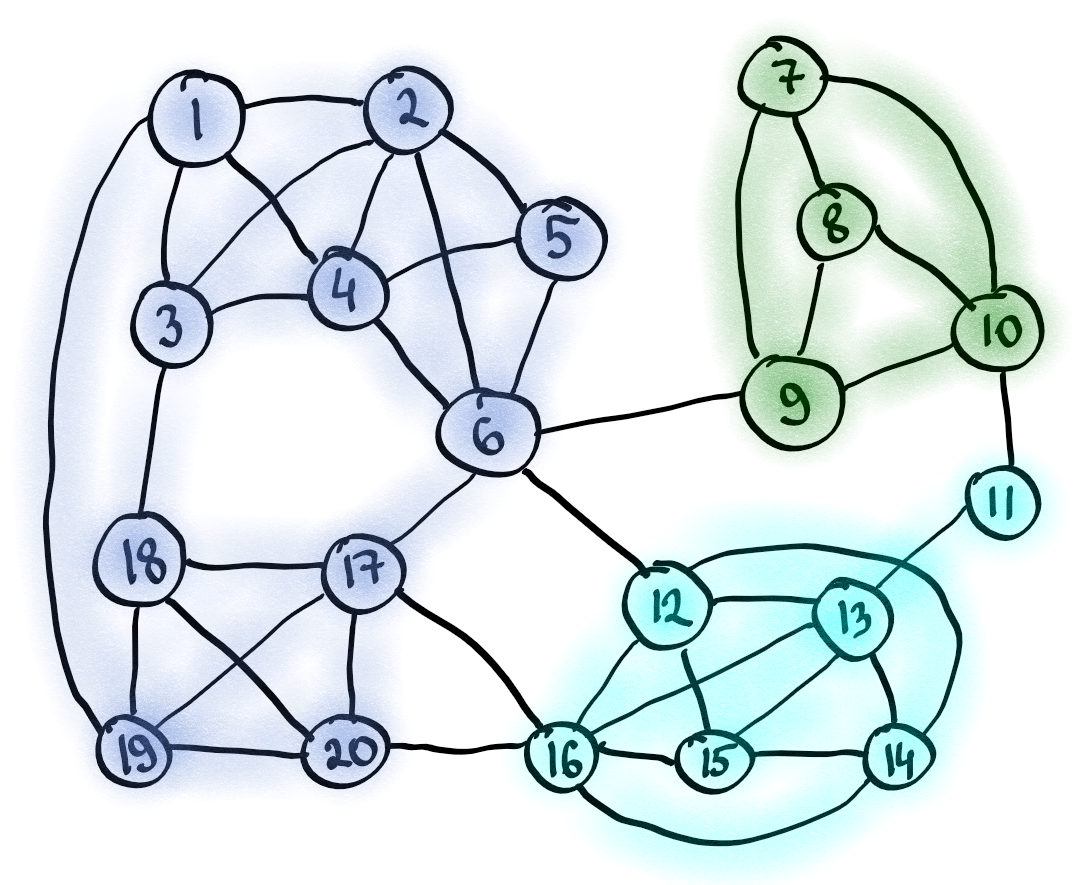
\includegraphics[width=0.4\textwidth]{1(3).png}
\end{figure} \\
Может показаться, что левая группа и группа справа снизу довольно сильные и будут только подбирать под себя другие, но здесь происходит кое-что интересное --- левая партия поджимает под себя правых нижних! Это произошло из-за того, что правые нижние хоть и были кластером тяжелее, чем кластер (7-8-9-10-11), но они сильнее связаны с левыми, нежели обособленный кластер (7-8-9-10-11), который связан с левым только через связь 6-9. Поэтому получаем такую картину:
\begin{figure}[h]
    \centering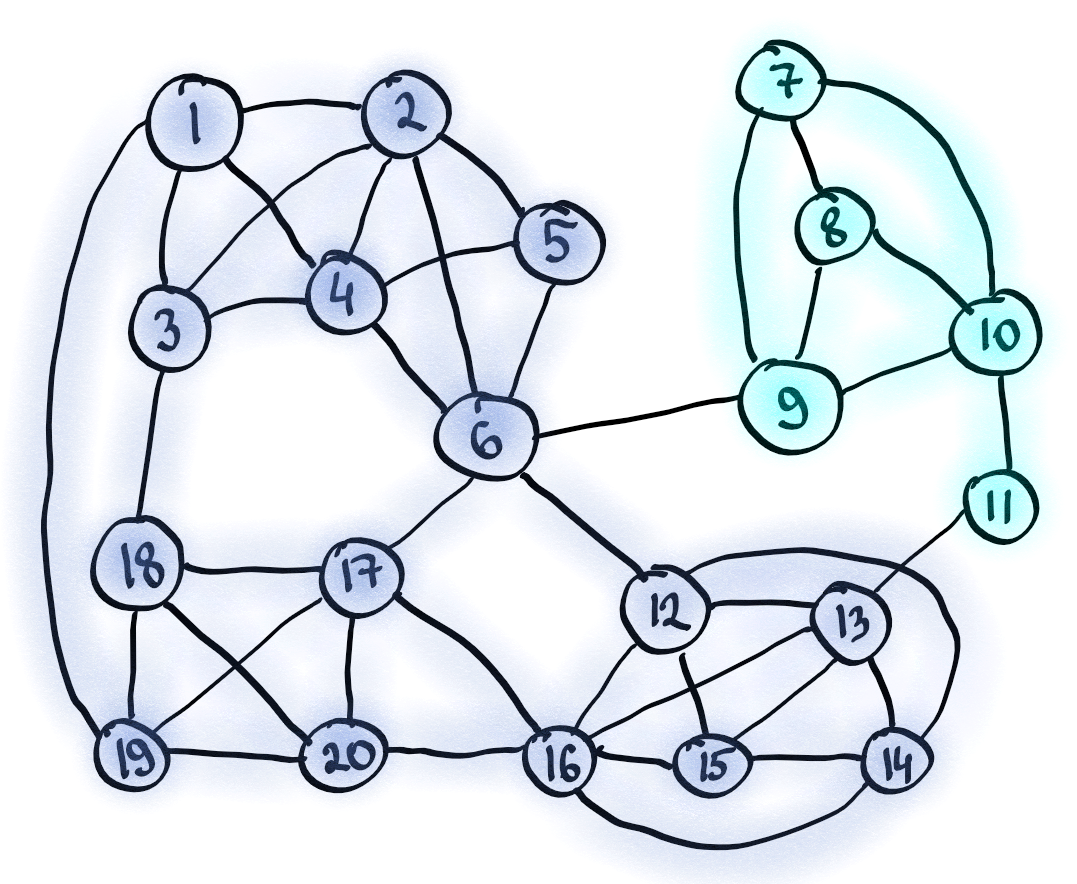
\includegraphics[width=0.4\textwidth]{1(2).png}
\end{figure}

\pagebreak\noindent Итак, мы понаблюдали, как кластеры могут легко захватывать другие кластеры при уменьшении порядка кластеризации и как вообще работает кластеризация. Но почему же это всё работает через собственные вектора и матрицу Лапласа?
\subsubsection*{\centering Вывод}
Дело в том, что среди собственных векторов прячется один важный вектор --- вектор Фидлера или, говоря без имён, вектор с минимальным собственным числом, не считая 0, т.е. второй по счёту в матрице $V$. А вся матрица Лапласа в принципе по-другому называется матрицей Кирхгофа. Вектор Фидлера помогает разбить граф на два кластера: вершины, соответствующие номерам строк с положительным значением в векторе Фидлера, относятся к одному кластеру, а отрицательные --- к другому. Второй вектор работает относительного первого как вектор Фидлера\dots\ как и третий относительно второго, если нам нужно разбиение уже на три кластера --- вот такое открытие! Далее итеративно четвёртый становится вектором Фидлера для третьего вектора и так далее и тому подобное\dots\ Метод k-средних выявляет такие зависимости внутри точек и делит их на кластеры, причём он может работать с точками как 1D, 2D и 3D, так и больших размерностей пространств, которые нам трудно представить!

\subsection*{\centering Задание №2. Это мы, получается, делаем конкурента Яндекса?}
Ну что, снова Imagine Dragons? Да, именно. И на ваших глазах уже вырисовывается граф с 15-ю пронумерованными вершинами и 35-ю стрелочками:
\begin{figure}[h]
    \centering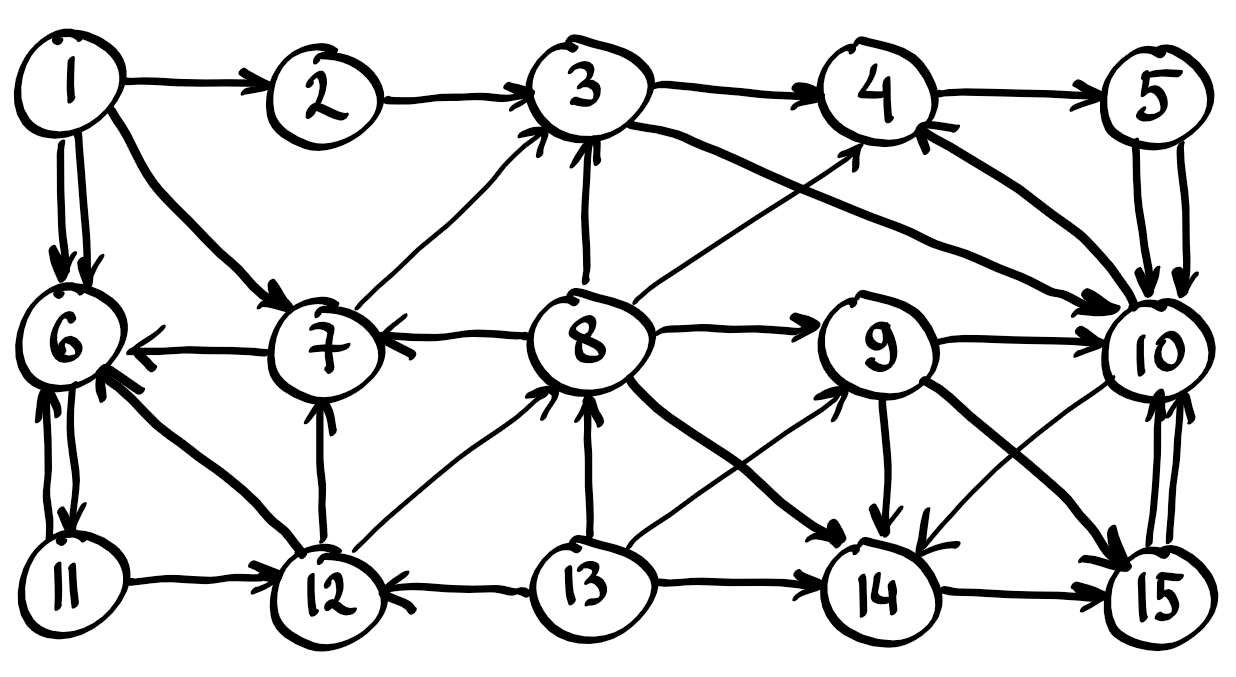
\includegraphics[width=0.5\textwidth]{2.png}
\end{figure}\\
Теперь нужно немного помучаться и составить матрицу $M$, которая составляется так, что каждый элемент матрицы $m_{ij} = \frac{\text{число стрелочек, выходящих из }j\text{-й вершины и входящих в }i\text{-ю вершину}}{\text{общее число стрелочек, выходящих из }j\text{-й вершины}}$. Затем приведу все дроби в красивый вид, чтобы получить красивую и громадную матрицу:
$$M = \left[ \begin{array}{ccccccccccccccc}
    \nicefrac{0}{4} & \nicefrac{0}{1} & \nicefrac{0}{2} & \nicefrac{0}{1} & \nicefrac{0}{2} & \nicefrac{0}{1} & \nicefrac{0}{2} & \nicefrac{0}{5} & \nicefrac{0}{3} & \nicefrac{0}{1} & \nicefrac{0}{2} & \nicefrac{0}{3} & \nicefrac{0}{4} & \nicefrac{0}{1} & \nicefrac{0}{2} \\
    \nicefrac{1}{4} & \nicefrac{0}{1} & \nicefrac{0}{2} & \nicefrac{0}{1} & \nicefrac{0}{2} & \nicefrac{0}{1} & \nicefrac{0}{2} & \nicefrac{0}{5} & \nicefrac{0}{3} & \nicefrac{0}{1} & \nicefrac{0}{2} & \nicefrac{0}{3} & \nicefrac{0}{4} & \nicefrac{0}{1} & \nicefrac{0}{2} \\
    \nicefrac{0}{4} & \nicefrac{1}{1} & \nicefrac{0}{2} & \nicefrac{0}{1} & \nicefrac{0}{2} & \nicefrac{0}{1} & \nicefrac{1}{2} & \nicefrac{1}{5} & \nicefrac{0}{3} & \nicefrac{0}{1} & \nicefrac{0}{2} & \nicefrac{0}{3} & \nicefrac{0}{4} & \nicefrac{0}{1} & \nicefrac{0}{2} \\
    \nicefrac{0}{4} & \nicefrac{0}{1} & \nicefrac{1}{2} & \nicefrac{0}{1} & \nicefrac{0}{2} & \nicefrac{0}{1} & \nicefrac{0}{2} & \nicefrac{1}{5} & \nicefrac{0}{3} & \nicefrac{1}{1} & \nicefrac{0}{2} & \nicefrac{0}{3} & \nicefrac{0}{4} & \nicefrac{0}{1} & \nicefrac{0}{2} \\
    \nicefrac{0}{4} & \nicefrac{0}{1} & \nicefrac{0}{2} & \nicefrac{1}{1} & \nicefrac{0}{2} & \nicefrac{0}{1} & \nicefrac{0}{2} & \nicefrac{0}{5} & \nicefrac{0}{3} & \nicefrac{0}{1} & \nicefrac{0}{2} & \nicefrac{0}{3} & \nicefrac{0}{4} & \nicefrac{0}{1} & \nicefrac{0}{2} \\
    \nicefrac{2}{4} & \nicefrac{0}{1} & \nicefrac{0}{2} & \nicefrac{0}{1} & \nicefrac{0}{2} & \nicefrac{0}{1} & \nicefrac{1}{2} & \nicefrac{0}{5} & \nicefrac{0}{3} & \nicefrac{0}{1} & \nicefrac{1}{2} & \nicefrac{1}{3} & \nicefrac{0}{4} & \nicefrac{0}{1} & \nicefrac{0}{2} \\
    \nicefrac{1}{4} & \nicefrac{0}{1} & \nicefrac{0}{2} & \nicefrac{0}{1} & \nicefrac{0}{2} & \nicefrac{0}{1} & \nicefrac{0}{2} & \nicefrac{1}{5} & \nicefrac{0}{3} & \nicefrac{0}{1} & \nicefrac{0}{2} & \nicefrac{1}{3} & \nicefrac{0}{4} & \nicefrac{0}{1} & \nicefrac{0}{2} \\
    \nicefrac{0}{4} & \nicefrac{0}{1} & \nicefrac{0}{2} & \nicefrac{0}{1} & \nicefrac{0}{2} & \nicefrac{0}{1} & \nicefrac{0}{2} & \nicefrac{0}{5} & \nicefrac{0}{3} & \nicefrac{0}{1} & \nicefrac{0}{2} & \nicefrac{1}{3} & \nicefrac{1}{4} & \nicefrac{0}{1} & \nicefrac{0}{2} \\
    \nicefrac{0}{4} & \nicefrac{0}{1} & \nicefrac{0}{2} & \nicefrac{0}{1} & \nicefrac{0}{2} & \nicefrac{0}{1} & \nicefrac{0}{2} & \nicefrac{1}{5} & \nicefrac{0}{3} & \nicefrac{0}{1} & \nicefrac{0}{2} & \nicefrac{0}{3} & \nicefrac{1}{4} & \nicefrac{0}{1} & \nicefrac{0}{2} \\
    \nicefrac{0}{4} & \nicefrac{0}{1} & \nicefrac{1}{2} & \nicefrac{0}{1} & \nicefrac{2}{2} & \nicefrac{0}{1} & \nicefrac{0}{2} & \nicefrac{0}{5} & \nicefrac{1}{3} & \nicefrac{0}{1} & \nicefrac{0}{2} & \nicefrac{0}{3} & \nicefrac{0}{4} & \nicefrac{0}{1} & \nicefrac{2}{2} \\
    \nicefrac{0}{4} & \nicefrac{0}{1} & \nicefrac{0}{2} & \nicefrac{0}{1} & \nicefrac{0}{2} & \nicefrac{1}{1} & \nicefrac{0}{2} & \nicefrac{0}{5} & \nicefrac{0}{3} & \nicefrac{0}{1} & \nicefrac{0}{2} & \nicefrac{0}{3} & \nicefrac{0}{4} & \nicefrac{0}{1} & \nicefrac{0}{2} \\
    \nicefrac{0}{4} & \nicefrac{0}{1} & \nicefrac{0}{2} & \nicefrac{0}{1} & \nicefrac{0}{2} & \nicefrac{0}{1} & \nicefrac{0}{2} & \nicefrac{0}{5} & \nicefrac{0}{3} & \nicefrac{0}{1} & \nicefrac{1}{2} & \nicefrac{0}{3} & \nicefrac{1}{4} & \nicefrac{0}{1} & \nicefrac{0}{2} \\
    \nicefrac{0}{4} & \nicefrac{0}{1} & \nicefrac{0}{2} & \nicefrac{0}{1} & \nicefrac{0}{2} & \nicefrac{0}{1} & \nicefrac{0}{2} & \nicefrac{0}{5} & \nicefrac{0}{3} & \nicefrac{0}{1} & \nicefrac{0}{2} & \nicefrac{0}{3} & \nicefrac{0}{4} & \nicefrac{0}{1} & \nicefrac{0}{2} \\
    \nicefrac{0}{4} & \nicefrac{0}{1} & \nicefrac{0}{2} & \nicefrac{0}{1} & \nicefrac{0}{2} & \nicefrac{0}{1} & \nicefrac{0}{2} & \nicefrac{1}{5} & \nicefrac{1}{3} & \nicefrac{0}{1} & \nicefrac{0}{2} & \nicefrac{0}{3} & \nicefrac{1}{4} & \nicefrac{0}{1} & \nicefrac{0}{2} \\
    \nicefrac{0}{4} & \nicefrac{0}{1} & \nicefrac{0}{2} & \nicefrac{0}{1} & \nicefrac{0}{2} & \nicefrac{0}{1} & \nicefrac{0}{2} & \nicefrac{0}{5} & \nicefrac{1}{3} & \nicefrac{0}{1} & \nicefrac{0}{2} & \nicefrac{0}{3} & \nicefrac{0}{4} & \nicefrac{1}{1} & \nicefrac{0}{2}
\end{array} \right] = \left[ \begin{array}{ccccccccccccccc}
    0 & 0 & 0 & 0 & 0 & 0 & 0 & 0 & 0 & 0 & 0 & 0 & 0 & 0 & 0 \\
    \nicefrac{1}{4} & 0 & 0 & 0 & 0 & 0 & 0 & 0 & 0 & 0 & 0 & 0 & 0 & 0 & 0 \\
    0 & 1 & 0 & 0 & 0 & 0 & \nicefrac{1}{2} & \nicefrac{1}{5} & 0 & 0 & 0 & 0 & 0 & 0 & 0 \\
    0 & 0 & \nicefrac{1}{2} & 0 & 0 & 0 & 0 & \nicefrac{1}{5} & 0 & 1 & 0 & 0 & 0 & 0 & 0 \\
    0 & 0 & 0 & 1 & 0 & 0 & 0 & 0 & 0 & 0 & 0 & 0 & 0 & 0 & 0 \\
    \nicefrac{1}{2} & 0 & 0 & 0 & 0 & 0 & \nicefrac{1}{2} & 0 & 0 & 0 & \nicefrac{1}{2} & \nicefrac{1}{3} & 0 & 0 & 0 \\
    \nicefrac{1}{4} & 0 & 0 & 0 & 0 & 0 & 0 & \nicefrac{1}{5} & 0 & 0 & 0 & \nicefrac{1}{3} & 0 & 0 & 0 \\
    0 & 0 & 0 & 0 & 0 & 0 & 0 & 0 & 0 & 0 & 0 & \nicefrac{1}{3} & \nicefrac{1}{4} & 0 & 0 \\
    0 & 0 & 0 & 0 & 0 & 0 & 0 & \nicefrac{1}{5} & 0 & 0 & 0 & 0 & \nicefrac{1}{4} & 0 & 0 \\
    0 & 0 & \nicefrac{1}{2} & 0 & 1 & 0 & 0 & 0 & \nicefrac{1}{3} & 0 & 0 & 0 & 0 & 0 & 1 \\
    0 & 0 & 0 & 0 & 0 & 1 & 0 & 0 & 0 & 0 & 0 & 0 & 0 & 0 & 0 \\
    0 & 0 & 0 & 0 & 0 & 0 & 0 & 0 & 0 & 0 & \nicefrac{1}{2} & 0 & \nicefrac{1}{4} & 0 & 0 \\
    0 & 0 & 0 & 0 & 0 & 0 & 0 & 0 & 0 & 0 & 0 & 0 & 0 & 0 & 0 \\
    0 & 0 & 0 & 0 & 0 & 0 & 0 & \nicefrac{1}{5} & \nicefrac{1}{3} & 0 & 0 & 0 & \nicefrac{1}{4} & 0 & 0 \\
    0 & 0 & 0 & 0 & 0 & 0 & 0 & 0 & \nicefrac{1}{3} & 0 & 0 & 0 & 0 & 1 & 0
\end{array} \right]$$

\pagebreak\noindent Смотрите, она даже не помещается на страницу и улетает немного за правую границу! Но это не важно, потому что сейчас мы будем искать для такой матрицы собственный вектор с максимальным собственным числом. И вот как он выглядит:
$$ \lambda = 1\quad v = \begin{pmatrix}
    0 \\ 0 \\ 0 \\ 1 \\ 1 \\ 0 \\ 0 \\ 0 \\ 0 \\ 1 \\ 0 \\ 0 \\ 0 \\ 0 \\ 0
\end{pmatrix}$$
Кажется, пока ничего интересного. В векторе три единички на 4-й, 5-й и 10-й строках. \\[1em] 
Но сейчас будет очень интересно --- мы воспользуемся следующим кодом:
\begin{figure}[h]
    \centering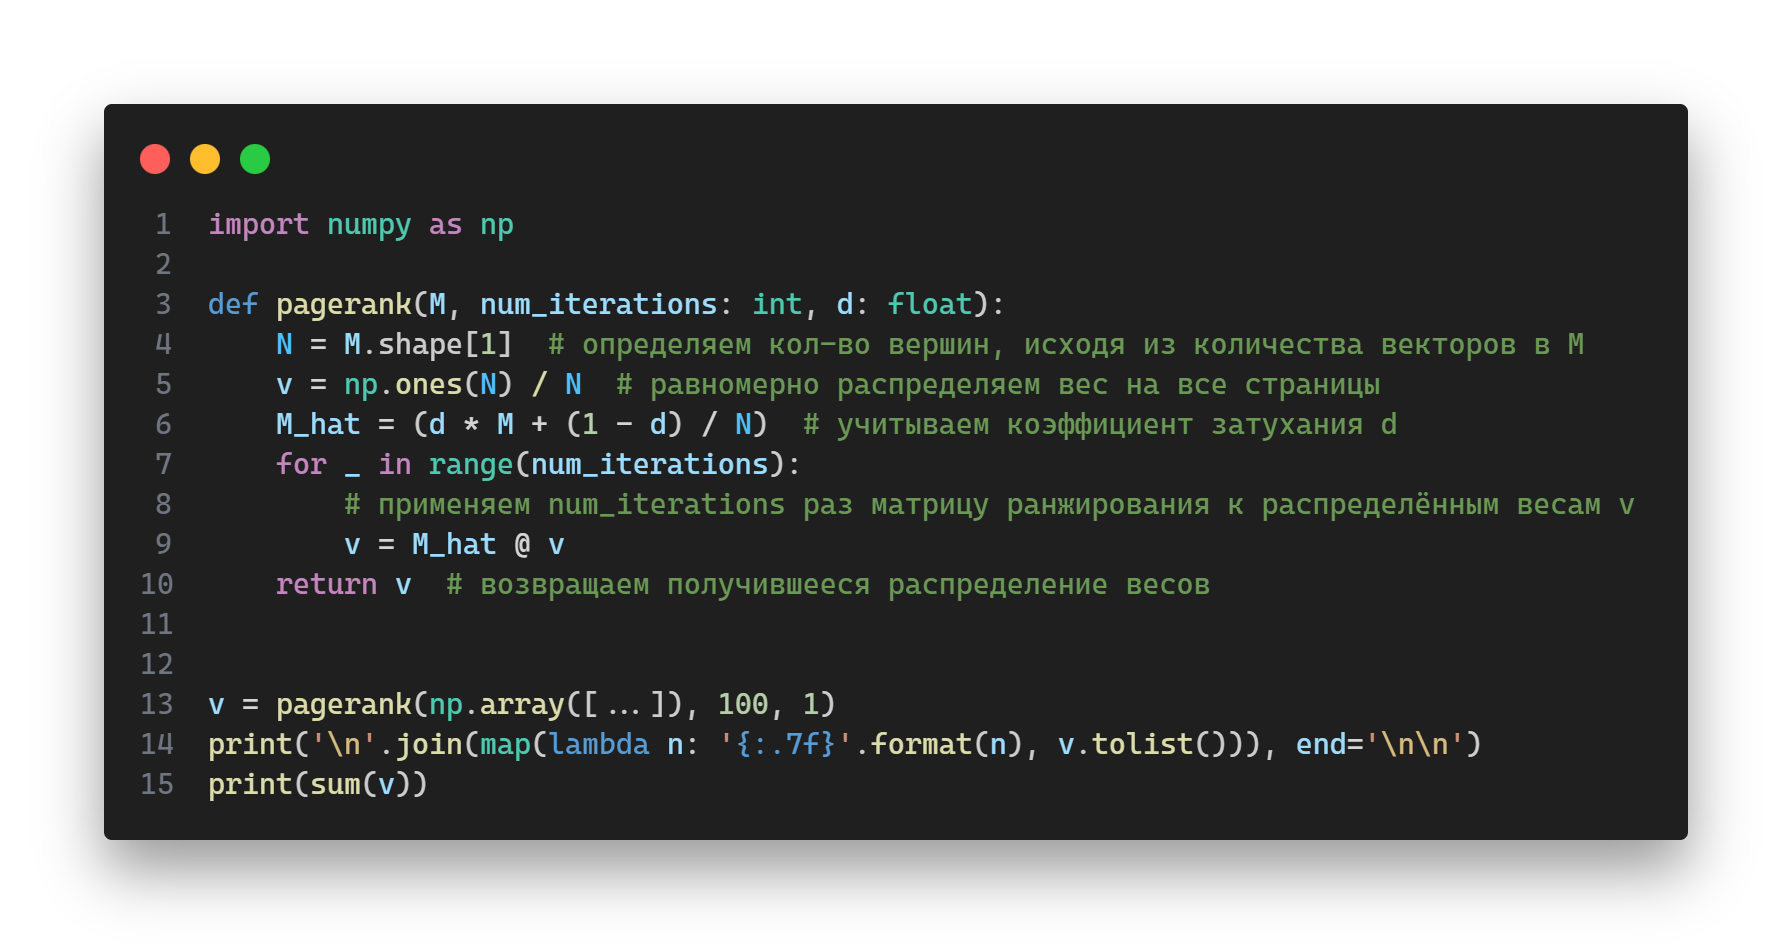
\includegraphics[width=0.6\textwidth]{2code.png}
\end{figure} \\
Просто импортируем \verb|numpy|, подгружаем всю матрицу весов в функцию \verb|pagerank()| (заменено на эллипсис в целях экономии пространства) вместе с количеством итераций \verb|num_iterations| и коэффициентом затухания \verb|d| и получаем \textbf{PageRank} для каждой страницы, которые показывают, как нужно ранжировать страницы. Остаётся вывести это всё в красивом виде и проверить, чему будет равна сумма всех рангов. Все комментарии, объясняющие алгоритм подробнее, оставлены в коде.\\[1em]
А теперь давайте взглянем на то, что нам выдаёт код для \verb|num_iterations| $= 100$ и \verb|d| $= 1$:
\begin{figure}[h]
    \centering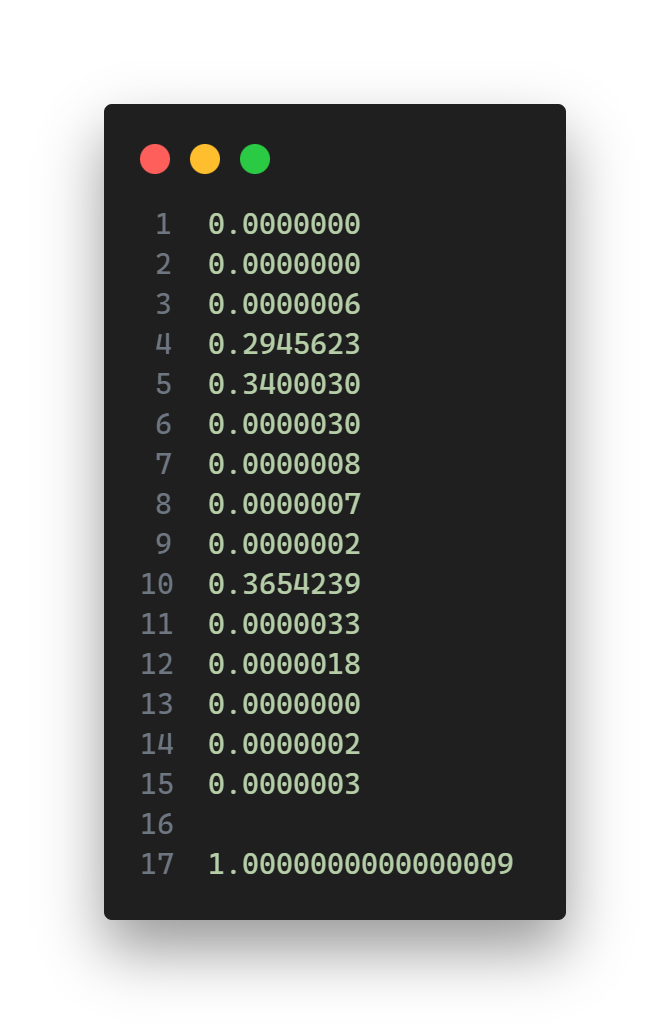
\includegraphics[width=0.21\textwidth]{output(1).png}
\end{figure}

\pagebreak\noindent Мы видим, что в большинстве строк очень малые значения, но в 4-й, 5-й и 10-й они сильно выделяются. \hypertarget{eigenvec_question}{Это ничего вам не напоминает?} Поговорим об этом в выводе\dots\ А сейчас наблюдаем, что сумма всех рангов равна единице (отображается погрешность, связанная с \href{https://0.30000000000000004.com}{проблемой <<0.30000000000000004>>}). Для такого ранжирования граф будет выглядеть так (чем больше и насыщеннее свечение вокруг вершины, тем выше она в ранжировании):
\begin{figure}[h]
    \centering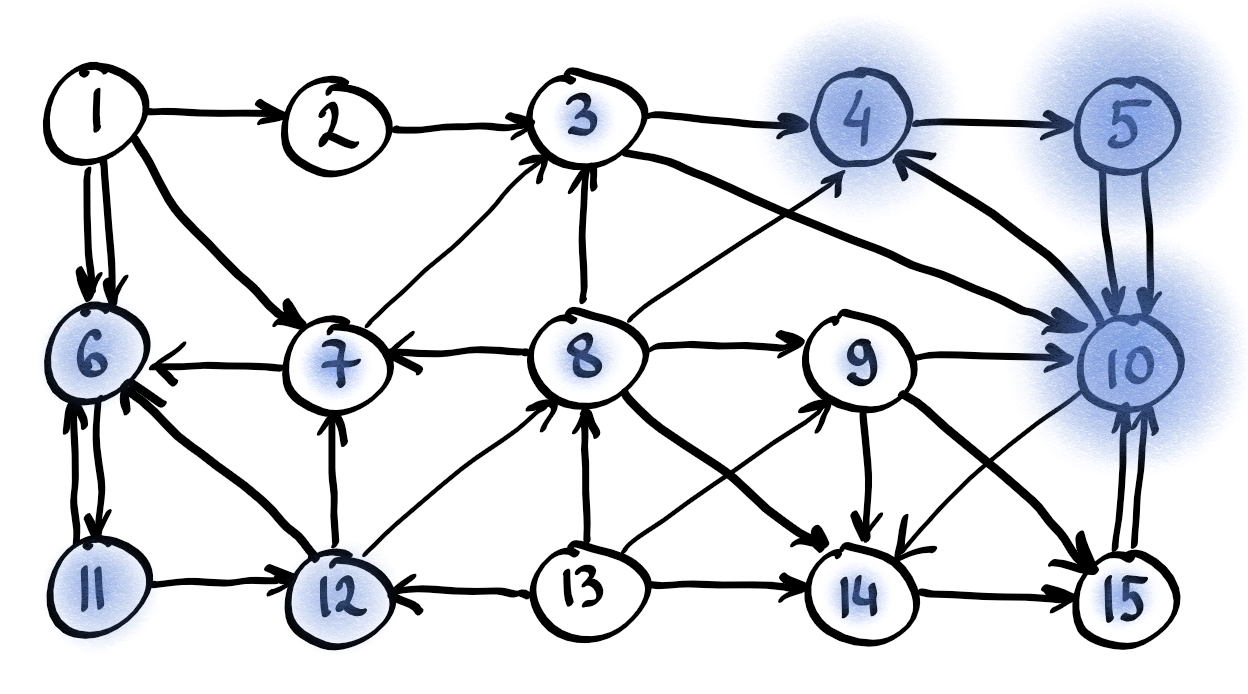
\includegraphics[width=0.5\textwidth]{2(1).png}
\end{figure}\\
Таким образом порядок ранжирования такой: \circled{10}-\circled{5}-\circled{4}-\circled{11}-\circled{6}-\circled{12}-\circled{7}-\circled{8}-\circled{3}-\circled{15}-\circled{14}-\circled{9}-\circled{1}-\circled{2}-\circled{13}. У последних трёх страниц ранг нулевой, поэтому их порядок не имеет значения и установлен по возрастанию номеров вершин.\\[1em]
Ну а сейчас взглянем на то, что нам выдаёт код для \verb|num_iterations| $= 100$ и \verb|d| $= 0.7$ (увеличим затухание):
\begin{figure}[h]
    \centering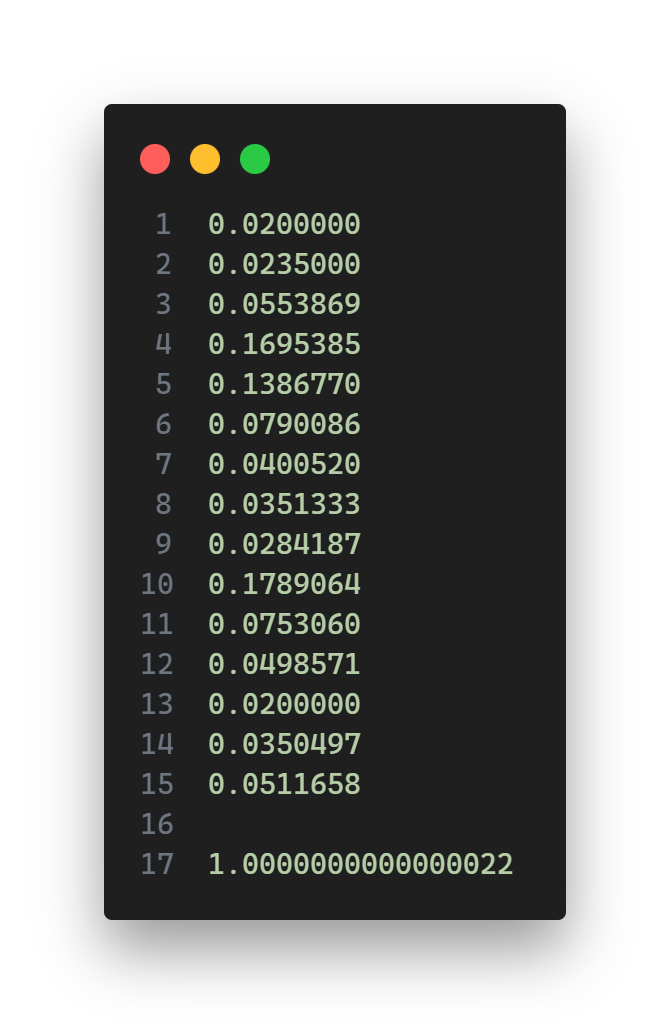
\includegraphics[width=0.21\textwidth]{output(0.7).png}
\end{figure} \\
Теперь картина несколько отличается от той, что была выше. Мы всё ещё видим, что 4-я, 5-я и 10-я вершины графа лидирующие, но другие страницы несколько приподнялись относительно 3-х лидеров и в общем и целом все страницы немного переранжировались. И на этот раз граф будет выглядеть следующим образом:
\begin{figure}[h]
    \centering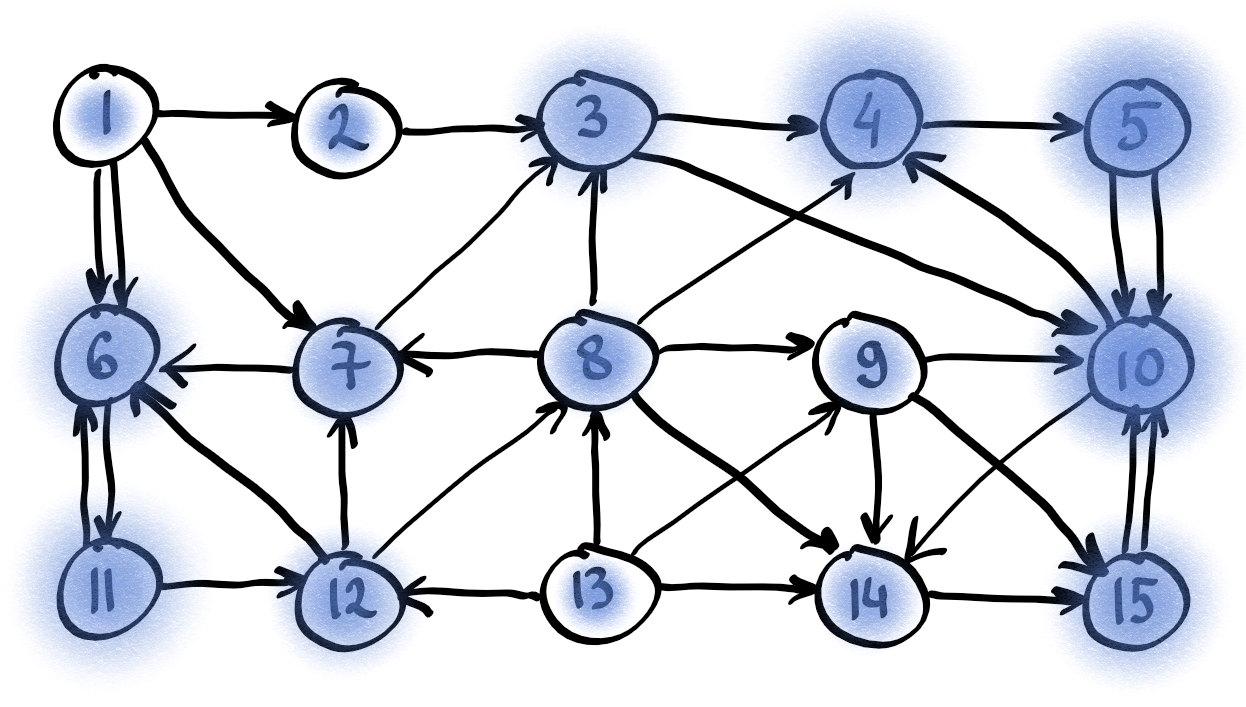
\includegraphics[width=0.5\textwidth]{2(0.7).png}
\end{figure}\\
Итак, порядок ранжирования таков: \circled{10}-\circled{4}-\circled{5}-\circled{6}-\circled{11}-\circled{3}-\circled{15}-\circled{12}-\circled{7}-\circled{8}-\circled{14}-\circled{9}-\circled{2}-\circled{1}-\circled{13}. Заметьте: несмотря на то, что \circled{1} ссылается на более авторитетные источники, чем \circled{13}, численный ранг у них одинаковый (1 по нумерации выше 13, поэтому порядок ранжирования такой, но численно их ранг ничем не отличаются). Вероятно, это один из минусов метода \textbf{PageRank}.

\subsubsection*{\centering Вывод}
Почему же всё так работает? Давайте обо всём по порядку. Матрица $M$ походит на матрицу марковского процесса --- в ней описано, с какой вероятностью пользователь, находясь на той или иной странице, перейдёт на следующую. И дальше на эту матрицу мы слева умножаем вектор $v$, где мы задаём не какую-то конкретную страницу, а равновероятно все сразу, чтобы предугадать, где пользователь окажется через 100 шагов, если начнёт не с какой-то конкретной страницы, а со всех одновременно. \\ А что показывает тот собственный вектор и почему я задавал \hyperlink{eigenvec_question}{тот вопрос}? На самом деле он показывает, куда стекаются в конечном итоге все вероятности --- другими словами, он показывает, какие страницы наиболее сильно влияют на рейтинг и занимают его львиную долю. И именно этот вектор показывает это, и никакой другой.\\ А что насчёт параметра $d$? Представьте человека, который живёт в деревне, где набрать воду можно только на краю деревни, но у него дырявое ведро. Он набрал воду и направился к себе домой, а по пути ему встречаются чужие дома с авторитетными и не очень жителями, с которыми обязательно захочется поговорить\dots\  и чем ближе $d$ к единице, тем больше этот человек напоминает студента, который, не останавливаясь на разговоры, спешит домой с дырявым ведром, чтобы принести туда как можно больше воды и не растерять её по пути. Но чем ближе $d$ к нулю, тем больше человек походит на старую бабушку, которая обязательно захочет остановиться у домов с авторитетными жителями (и тем более безразлично ей будет, авторитетные они или нет), чтобы поболтать с ними, потеряв у них очень много воды и донеся тем самым меньше воды до дома. Так вот дом человека --- те вершины, на которые указывается собственный вектор, вода --- каждый из весов вектора $v$ по отдельности, дома авторитетных жителей --- вершины, в которые стекается больше стрелок, чем в другие. Так и работает $d$: распределяет ранг с \circled{4}, \circled{5} и \circled{10} на другие не менее значимые страницы, например, \circled{6} или \circled{12}. И, если рассмотреть $d = 0$, то можно увидеть, как ранги распределились равномерно, как будто матрица $M$ совсем не действовала на вектор $v$.\\
А о том, какое отношение всё это имеет к марковским процессам, я рассказал ещё в первом абзаце --- матрица $M$ является матрицей вероятностей, а вектор $v$ есть вектор вероятностей.
\end{document}